\documentclass{article}
\usepackage[english]{babel}
\usepackage[utf8]{inputenc}
\usepackage[T1]{fontenc}
\usepackage[a4paper]{geometry}
\usepackage{amsmath}
\usepackage{graphicx}
\usepackage{glossaries}
\usepackage{listings}
\usepackage{xcolor}
\usepackage{amssymb}

\geometry{textwidth=14cm}

\makeglossaries

\newglossaryentry{Benzodiazepines}
{
name=Benzodiazepines,
description={(BZD, BDZ, BZs), sometimes called "benzos", are a class of psychoactive drugs whose core chemical structure is the fusion of a benzene ring and a diazepine ring.[2]Familiar names include Valium and Xanax.[1]}
}
\newglossaryentry{Alprazolam}
{
name=Alprazolam,
description={}
}
\newglossaryentry{Triazolam}
{
name=Triazolam,
description={}
}
\newglossaryentry{Placebo}
{
name=Placebo,
description={}
}

\title{My title goes here}
\author{Filip Paskalev S19155623}

% Document
\begin{document}



    %%%%%%%%%%%%%%%%%%%%%%%%%%%%%%%%%%%%%%%%%%%%%%
    % Title page
    %%%%%%%%%%%%%%%%%%%%%%%%%%%%%%%%%%%%%%%%%%%%%%


    \begin{titlepage}
        \begin{center}
            \vspace{0.5cm}
            \LARGE
            
\includegraphics[width=0.5\textwidth]{images/bcu-logo-rectangle.png}\\
            FACULTY OF COMPUTING ENGINEERING AND THE BUILT ENVIRONMENT\\
            \vspace{0.5cm}
            \large
            MSc. Advanced Computer Science
            \vspace{1cm}
            \vspace{0.5cm}
            Research\\
            \Huge
            An experiment on the effects of the anti-anxiety drug on memory recovery
            \vspace{0.5cm}
        \end{center}
        \vspace*{\fill}
        \raggedcenter
        Module Leader: Yevgeniya Kovalchuk
        \vspace{0.2cm}\\
        Module: Advanced Data Science\\
        Code: CMP7161\\
        Student: Filip Paskalev \\
        \cyrchar\textnumero{} S19155623
        \vspace{0.125cm}\\
        \begin{center}
            \vspace{1cm}
            Academic year 2019/2020
        \end{center}
    \end{titlepage}

    \newpage

    \makeglossary
    \newpage

    \makeindex
    \tableofcontents
    \listoffigures
    \listoftables
    \newpage

    \begin{abstract}
        The report is over an experiment on the effects of anti-anxiety medicament on memory recall when being primed with happy or sad memories. The focus of the analysis is on the placebo effect and the effect of anti-anxiety medicine on memory recall.
        Data set is created from the data of participants in the experiment, done on novel Islanders who mimic real-life humans in response to external factors.
        The experiment was executed under the supervision of Mr. Almohalwas at UCLA. All aspects of the experiment such as experimental design, data collection, and preprocessing were done from Steve Ahn.
    \end{abstract}
    \newpage


    %%%%%%%%%%%%%%%%%%%%%%%%%%%%%%%%%%%%%%%%%%%%%%
    % Introduction
    %%%%%%%%%%%%%%%%%%%%%%%%%%%%%%%%%%%%%%%%%%%%%%


    \section{Introduction}\label{sec:introduction}
    \subsection{Background}\label{subsec:background}
    \subsubsection{Building the Case}
    \paragraph{Anti-Anxiety Medicine}
    Obstructive effects of Benzodiazepines:\\
    Long term adverse effects on Long Term Potentiation of synapses, metacognition and memory recall ability юю
    http://www.jstor.org/stable/43854146
    \paragraph{Happy Memories}
    Research showed positive memories to have a deeper and greater volume of striatum representation under an \\
    fMRI https://www.sciencedirect.com/science/article/pii/S0896627314008484
    \paragraph{Sad Memories}
    Research shown sad memories invoke better memory recall for evolutionary \\
    purpose whereas, happy memories are more susceptible to false memories \\
    http://www.jstor.org/stable/40064315
    \subsubsection{Participants}
    All genders above 25+ years old to ensure a fully developed pre-frontal cortex, a region responsible for higher-level cognition and memory recall.
    \subsection{Aim and objectives}\label{subsec:aim-and-objectives}
    \begin{enumerate}
        \item     General observations and analysis of effective Benzodiazepines?
        \item     Does the anti-anxiety drug work differently at different ages?
        \item     To establish the effect of placebo and its correlation with the subject.
        \begin{itemize}
            \item If there is a placebo effect to analyze at what point it occurs.
        \end{itemize}
        \item     Does anxiety medicine drugs have an effect on memory?
        \item     To analyze whether there are an influence and connection between the application of positive or negative emotions before taking the drug.
    \end{enumerate}
    \newpage


    %%%%%%%%%%%%%%%%%%%%%%%%%%%%%%%%%%%%%%%%%%%%%%
    % Data set
    %%%%%%%%%%%%%%%%%%%%%%%%%%%%%%%%%%%%%%%%%%%%%%


    \section{Data set}
    \subsection{Description}
    Data containing Islander general, drug, and test information.\\
    \\
    Columns:\\
    \begin{longtable}{ l p{3in} }
        first_name: & First name of Islander.\\
        last_name: & Last name of Islander.\\
        age: & Age of Islander.\\
        Happy_Sad_group: & Happy or Sad Memory priming block.\\
        Dosage: & 1-3 to indicate the level of dosage (low - medium - over recommended daily intake).\\
        Drug: & Type of Drug administered to Islander.\\
        Mem_Score_Before: & Seconds - how long it took to finish a memory test before drug exposure.\\
        Mem_Score_After: & Seconds - how long it took to finish a memory test after addiction achieved.\\
        Diff: & Seconds - difference between memory score before and after.\\
    \end{longtable}
    \subsection{Preparing data}
    \paragraph{Loading libraries}
    Importing all the libraries that will be needed for the project.
    \begin{lstlisting}[language=Python]
        # math tools
        import numpy as np
        # import and manage data sets
        import pandas as pd
        # visualization & sub libarary with tool for visualization
        import matplotlib.pyplot as plt

        import sklearn
        # for splitting the data set
        from sklearn.model_selection import train_test_split
        # label encoding the data
        from sklearn.preprocessing import LabelEncoder
        # importing one hot encoder from sklearn
        from sklearn.preprocessing import OneHotEncoder

        from sklearn.utils import shuffle
    \end{lstlisting}
    \newpage
    \subsection{Sample}
    \begin{figure}[!htb]
        \center{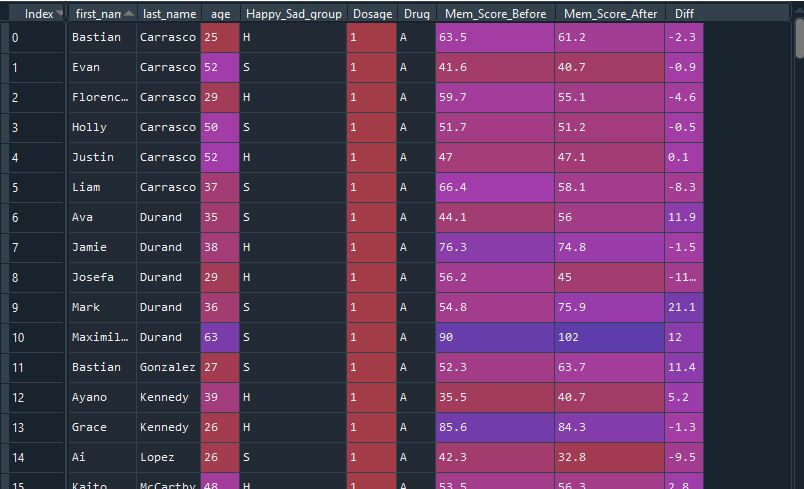
\includegraphics[width=10cm]{figures/raw_data_analysis_01.JPG}}
        \caption{\label{fig:raw-data-sample} Raw data sample}
    \end{figure}
    \newpage
    \subsection{Information}
    \subsubsection{Field types} Check what type are the fields in the data.
    \begin{lstlisting}[language=Python]
        source.info()
    \end{lstlisting}
    \paragraph{Result} Visualization of the result.
    \begin{lstlisting}[language=Python]
        RangeIndex: 198 entries, 0 to 197
        Data columns (total 9 columns):
        # Column Non-Null Count Dtype
        --- ------ -------------- -----
        0 first_name 198 non-null object
        1 last_name 198 non-null object
        2 age 198 non-null int64
        3 Happy_Sad_group 198 non-null object
        4 Dosage 198 non-null int64
        5 Drug 198 non-null object
        6 Mem_Score_Before 198 non-null float64
        7 Mem_Score_After 198 non-null float64
        8 Diff 198 non-null float64
        dtypes: float64(3), int64(2), object(4)
        memory usage: 14.0+ KB
    \end{lstlisting}
    \subsubsection{NULL's} Check if data have any NULL values or missing values.
    \begin{lstlisting}[language=Python]
        print(source.isnull().sum())
    \end{lstlisting}
    \paragraph{Result} Visualization of the result.
    \begin{lstlisting}[language=Python]
        first_name 0
        last_name 0
        age 0
        Happy_Sad_group 0
        Dosage 0
        Drug 0
        Mem_Score_Before 0
        Mem_Score_After 0
        Diff 0
        dtype: int64
    \end{lstlisting}
    \subsubsection{Describe} Brief summary data description.
    \begin{lstlisting}[language=Python]
        print(source.describe())
    \end{lstlisting}
    \paragraph{Result} Visualization of the result.
    \begin{lstlisting}[language=Python]
        age Dosage MSB MSA Diff
        count 198.000000 198.000000 198.000000 198.000000 198.000000
        mean 39.530303 1.989899 57.967677 60.922222 2.954545
        std 12.023099 0.818504 15.766007 18.133851 10.754603
        min 24.000000 1.000000 27.200000 27.100000 -40.400000
        25%   30.000000  1.000000   46.525000  47.175000  -3.175000
        50%   37.000000  2.000000   54.800000  56.750000  1.700000
        75%   48.000000  3.000000   68.400000  73.250000  5.925000
        max 83.000000 3.000000 110.000000 120.000000 49.000000
    \end{lstlisting}
    \subsection{Analysis}
    \paragraph{}
    Data don't contain any NULL values or any missing values.
    All the attributes will be usable.
    Field[1] "first\_name" and "last\_name" can be concatenate in one field - "name".
    Types of the field "age", "Dosage", "second\_name", should be optimized in a smaller unit.
    "Happy\_Sad\_group" and "Drug" need to be grouped by type.
    \newpage



    %%%%%%%%%%%%%%%%%%%%%%%%%%%%%%%%%%%%%%%%%%%%%%
    % Pre-processing
    %%%%%%%%%%%%%%%%%%%%%%%%%%%%%%%%%%%%%%%%%%%%%%


    \section{Pre-processing}
    \subsection{Trim}
    For the purpose of the study, we do not need the fields - first name and second name. They will be combined into one, as shown in the following lines.
    \begin{lstlisting}[language=Python]
        # Combine "first_name" and "last_name" field
        in one field with label name
        data["name"] = data["first_name"] + " " + data["last_name"]
        # Remove column first_name
        del data['first_name']
        # Remove column last_name
        del data['last_name']
    \end{lstlisting}
    \subsection{Fiels drug}
    Label field "Drug" by labels:
    \begin{itemize}
        \item A (Alprazolam) = 0
        \item T (Triazolam) = 1
        \item S (Sugar Tablet - Placebo) = 2
    \end{itemize}
    The function takes and add a string for parameters.
    Later they will be converted in integers.
    \begin{lstlisting}[language=Python]
        # Iterate over data and label all data with correct labels
        data['Drug'] = data['Drug'].str.replace('A', '0', case = False)
        data['Drug'] = data['Drug'].str.replace('T', '1', case = False)
        data['Drug'] = data['Drug'].str.replace('S', '2', case = False)
    \end{lstlisting}
    \subsection{Field Happy\_Sad\_group}
    In the same methodological field "Happy\_Sad\_group" will be labeled -
    \begin{itemize}
        \item H (Happy) = 0
        \item S (Sad) = 1
    \end{itemize}
    The field is in a string, later it will be converted in integers.
    \begin{lstlisting}[language=Python]
        data['Happy_Sad_group'] =
            data['Happy_Sad_group'].str.replace('H', '0', case = False)
        data['Happy_Sad_group'] =
            data['Happy_Sad_group'].str.replace('S', '1', case = False)
    \end{lstlisting}
    \newpage
    \subsection{String fields}
    \paragraph{Localization fields}
    Localization which fields need to be handled by casting to integers.
    \begin{lstlisting}[language=Python]
        data.info()
    \end{lstlisting}
    \paragraph{Result}
    Visualization of the result from the check.
    \begin{lstlisting}[language=Python]
        RangeIndex: 198 entries, 0 to 197
        Data columns (total 8 columns):
        # Column Non-Null Count Dtype
        --- ------ -------------- -----
        0 age 198 non-null int64
        1 Happy_Sad_group 198 non-null object
        2 Dosage 198 non-null int64
        3 Drug 198 non-null object
        4 Mem_Score_Before 198 non-null float64
        5 Mem_Score_After 198 non-null float64
        6 Diff 198 non-null float64
        7 name 198 non-null object
        dtypes: float64(3), int64(2), object(3)
    \end{lstlisting}
    \subsubsection{Casting}
    Converting the fields.
    \begin{lstlisting}[language=Python]
        data['Drug'] = data['Drug'].astype(int)
        data['Happy_Sad_group'] = data['Happy_Sad_group'].astype(int)
    \end{lstlisting}
    \paragraph{Result}
    Visualization of the result from casting.
    \begin{lstlisting}[language=Python]
        RangeIndex: 198 entries, 0 to 197
        Data columns (total 8 columns):
        # Column Non-Null Count Dtype
        --- ------ -------------- -----
        0 age 198 non-null int64
        1 Happy_Sad_group 198 non-null int32
        2 Dosage 198 non-null int64
        3 Drug 198 non-null int32
        4 Mem_Score_Before 198 non-null float64
        5 Mem_Score_After 198 non-null float64
        6 Diff 198 non-null float64
        7 name 198 non-null object
        dtypes: float64(3), int32(2), int64(2), object(1)
        memory usage: 11.0+ KB
    \end{lstlisting}
    \newpage
    \subsection{Field age\_group}
    \paragraph{Purpose}
    Create an additional field that will be used for the purpose of analysis in the study. The group will be separated on four[1] -
    \begin{itemize}
        \item child (under 15) = 0
        \item young adult (16 - 30) = 1
        \item middle-aged adult (31 - 50) = 2
        \item senior adult (over 50) = 3
    \end{itemize}
    \paragraph{Code} Preview of the steps for creating the new field.
    \begin{lstlisting}[language=Python]
        # Create obj age_group and fill it with
        categorizated data from column age
        age_group = []
        # Grouping the ages 0-15, 16-30, 30-50 , 51-max
        for i in data.itertuples():
        index = 0
        if i[1] <= 15:
        age_group.append(0)
        elif i[1] <= 30:
        age_group.append(1)
        elif i[1] <= 50:
        age_group.append(2)
        else:
        age_group.append(3)
        index = index + 1
        # Add columnto the data
        data['age_group'] = age_group
    \end{lstlisting}
    \paragraph{Result}
    Visualization of the result.
    \begin{lstlisting}[language=Python]
        angeIndex: 198 entries, 0 to 197
        Data columns (total 9 columns):
        # Column Non-Null Count Dtype
        --- ------ -------------- -----
        0 age 198 non-null int64
        1 Happy_Sad_group 198 non-null int32
        2 Dosage 198 non-null int64
        3 Drug 198 non-null int32
        4 Mem_Score_Before 198 non-null float64
        5 Mem_Score_After 198 non-null float64
        6 Diff 198 non-null float64
        7 name 198 non-null object
        8 age_group 198 non-null int64
        dtypes: float64(3), int32(2), int64(3), object(1)
        memory usage: 12.5+ KB
    \end{lstlisting}
    \newpage
    \subsection{Encoder}
    \subsubsection{Field name}
    Creating an object of type LabelEncoder() which will encode all names in the field "name".
    \begin{lstlisting}[language=Python]
        label_encoder = LabelEncoder()
        data['name']= label_encoder.fit_transform(data['name'])
    \end{lstlisting}
    \subsubsection{Rest of the fields}
    Using objects from the previous paragraph, and use the same methodology to encode the rest of the fields.
    The fields are already in a numerical category, but if some of the categories missing
    (Example "ages\_group" - the data don't contain group 0 - children)
    recategorization is possible for optimization.
    This will help for better automatization of the code structure in the future.
    \begin{lstlisting}
        data['age_group']= label_encoder.fit_transform(data['age_group'])
        data['Drug']= label_encoder.fit_transform(data['Drug'])
        data['Happy_Sad_group']= label_encoder.fit_transform(data['Happy_Sad_group'])
    \end{lstlisting}
    \subsection{Optimization}
    \subsubsection{int64 to int32}
    Optimize the size of the stored types in the field.
    This step is not necessary, but it will be a helpful feature if the training model data grow.
    \begin{lstlisting}[language=Python]
        data['Dosage'] = data['Dosage'].astype(int)
        data['age'] = data['age'].astype(int)
        data['age_group'] = data['age_group'].astype(int)
    \end{lstlisting}
    \subsubsection{Cleaning unused objects}
    Clean all the objects that have been used to now for better optimization and cleaner code.
    Variable "i" is used temporarily, and it doesn't need to be store.
    Object "age\_group is stored in object "data", and it doesn't need to have a copy of it.
    Object "label\_encoder", has finished its purpose, it doesn't need to be saved.
    \begin{lstlisting}[language=Python]
        del age_group
        del i
        del label_encoder
    \end{lstlisting}
    \newpage

    %%%%%%%%%%%%%%%%%%%%%%%%%%%%%%%%%%%%%%%%%%%%%%
    % Simple linear regression
    %%%%%%%%%%%%%%%%%%%%%%%%%%%%%%%%%%%%%%%%%%%%%%

    \section{Simple Linear Regression}
    Building the Simple linear regression model, based on data set.
    \subsection{Import} Importing needable libraries
    \begin{lstlisting}[language=Python]
        import numpy as np
        import pandas as pd
        import sklearn
        from sklearn import linear_model
        import pickle
        import matplotlib.pyplot as plt
    \end{lstlisting}
    \subsection{Load}
    Loading the data.
    Shuffling the data is optional.
    Not every fields are inserted in to the data, fields are
    inserted base on what will be investigated and the relation
    between them and target.
    \begin{lstlisting}[language=Python]
        data = pd.read_csv('data.csv')
        from sklearn.utils import shuffle
        data = shuffle(data)
        data = data[[
        "Happy_Sad_group",
        "Dosage",
        "Drug",
        "Mem_Score_Before",
        "Mem_Score_After",
        "age_group"]]
    \end{lstlisting}
    \subsection{Prediction}
    Targeting the prediction field.
    \begin{lstlisting}[language=Python]
        predict = "Mem_Score_After"
        x = np.array(data.drop([predict], 1))
        y = np.array(data[predict])
    \end{lstlisting}
    \subsection{Split}
    Preraring data to train and split data lfor tests.
    \begin{lstlisting}[language=Python]
x_train, x_test, y_train, y_test =
    sklearn.model_selection.train_test_split(
        x, y, test_size = 0.1, random_state = 0)
    \end{lstlisting}
    \subsection{Train}
    Train the model.
    Pickle module is ised to save the model.
    \begin{lstlisting}[language=Python]
        best = 0
        for _ in range(10000):
        x_train, x_test, y_train, y_test =
            sklearn.model_selection.train_test_split(x, y, test_size=0.1)
        linear = linear_model.LinearRegression()
        linear.fit(x_train, y_train)
        acc = linear.score(x_test, y_test)
        print(acc)
        if acc > best:
        best = acc
        with open("simple_linear_regression.pickle", "wb") as f:
        pickle.dump(linear, f)
        pickle_in = open("simple_linear_regression.pickle", "rb")
        linear = pickle.load(pickle_in)
        predicted = linear.predict(x_test)
        for x in range(len(predicted)):
        print(predicted[x], x_test[x], y_test[x])
    \end{lstlisting}
    \newpage

    %%%%%%%%%%%%%%%%%%%%%%%%%%%%%%%%%%%%%%%%%%%%%%
    % Random Forest Regression
    %%%%%%%%%%%%%%%%%%%%%%%%%%%%%%%%%%%%%%%%%%%%%%


    \section{Random Forest Regression}
    Building the Random Forest Regression model, based on data set.
    \subsection{Build} Importing needable libraries
    \begin{lstlisting}[language=Python]
        import numpy as np
        import pandas as pd
        import sklearn as sklearn
        from sklearn import linear_model
        from sklearn.ensemble import RandomForestRegressor
        from sklearn.utils import shuffle
        import pickle
        import matplotlib.pyplot as plt
        import seaborn as sns
        from sklearn.metrics import r2_score
        from sklearn.ensemble import RandomForestRegressor
    \end{lstlisting}
    \subsection{Load}
    Loading the data. On the same methodological like on linear regression data is load.
    \begin{lstlisting}[language=Python]
        data = pd.read_csv('data.csv')
        data = shuffle(data)
        data = data[[
        "age",
        "Happy_Sad_group",
        "Dosage",
        "Drug",
        "Mem_Score_Before",
        "Mem_Score_After",
        "Diff",
        "name",
        "age_group"
        ]]
        predict = "Mem_Score_After"
        x = np.array(data.drop([predict], 1))
        y = np.array(data[predict])
    \end{lstlisting}
    \newpage
    \subsection{Split}
    Split the data on train sets and save 10\% from it for tests.
    \begin{lstlisting}[language=Python]
        x_train, x_test, y_train, y_test =
            sklearn.model_selection.train_test_split(
                x, y, test_size = 0.1, random_state = 0)
    \end{lstlisting}
    \subsection{Train}
    Train the model.
    Pickle module is used to save the model.
    \begin{lstlisting}[language=Python]
        best = 0
        for _ in range(10):
        x_train, x_test, y_train, y_test =
            sklearn.model_selection.train_test_split(
                x, y, test_size=0.1)

        forest = RandomForestRegressor()

        forest.fit(x_train, y_train)
        acc = forest.score(x_test, y_test)
        print(acc)

        if acc > best:
        best = acc
        with open("random_forest_regression.pickle", "wb") as f:
        pickle.dump(forest, f)
    \end{lstlisting}
    \newpage


    %%%%%%%%%%%%%%%%%%%%%%%%%%%%%%%%%%%%%%%%%%%%%%
    % Explore data
    %%%%%%%%%%%%%%%%%%%%%%%%%%%%%%%%%%%%%%%%%%%%%%


    \section{Explore}
    \subsection{Correlation}
    \paragraph{}
    Correlation between features and target.
    \begin{lstlisting}[language=Python]
        correlation = data.corr()
        plt.figure(figsize=(10,8))
        heatmap = sns.heatmap(correlation,
                              annot=True,
                              linewidths=1,
                              vmin=1)
    \end{lstlisting}
    \begin{figure}[!htb]
        \center{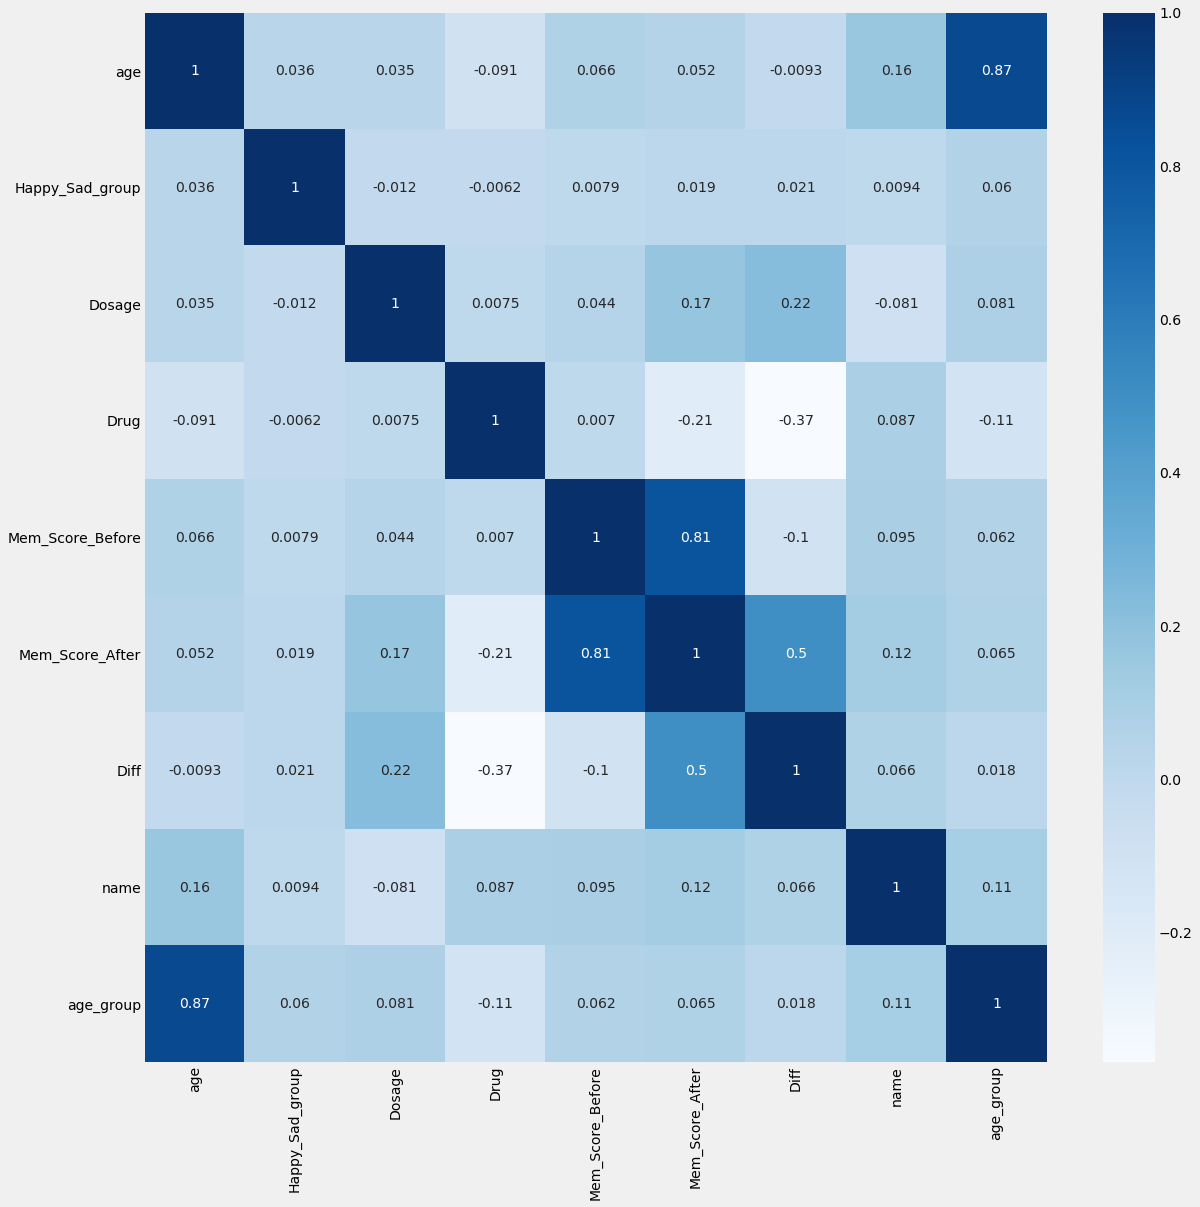
\includegraphics[width=10cm]{figures/correlation.png}}
        \caption{\label{fig:correlation} Finding correlation visualization}
    \end{figure}
    \newpage
    \subsection{Memory score after medicament}
    \paragraph{}
    General view of the memory score of the subjects after effect of drugs.
    \begin{figure}[!htb]
        \center{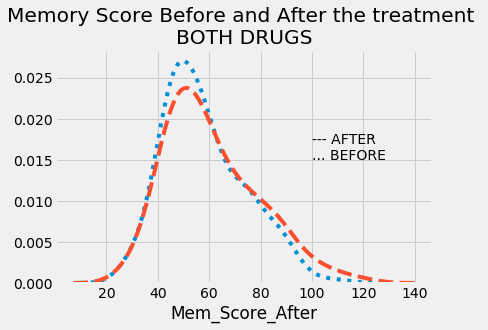
\includegraphics[width=10cm]{figures/msa-general-view.png}}
        \caption{\label{fig:msa-general-view} Memory score after drug}
    \end{figure}
    \subsection{Dosage effect}
    \paragraph{}
    Visualization memory score based on the effect of the dosage.
    Drugs are represented in 3 groups.
    \begin{figure}[!htb]
        \center{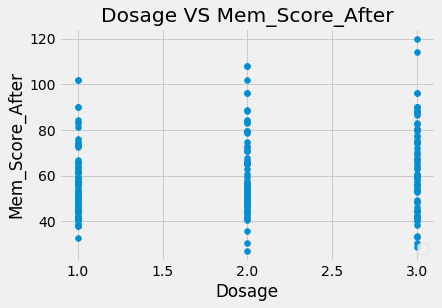
\includegraphics[width=10cm]{figures/dossage-effect.png}}
        \caption{\label{fig:dossage-effect} Effect of dosage}
    \end{figure}
    \subsection{Age analysis}
    \paragraph{}
    Visual representing of age groups of tested subjects.
    \begin{figure}[!htb]
        \center{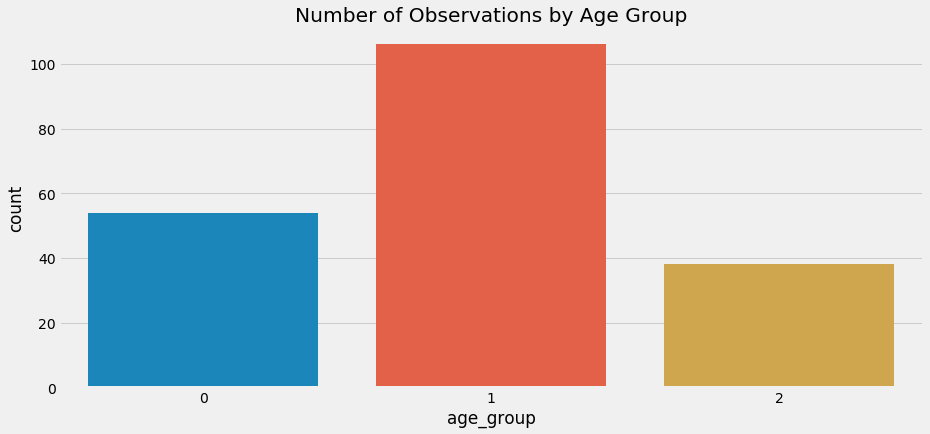
\includegraphics[width=10cm]{figures/age-groups-general-view.png}}
        \caption{\label{fig:age-groups-general-view} Age groups}
    \end{figure}
    \paragraph{}
    Visual of age groups of tested subjects.
    \begin{figure}[!htb]
        \center{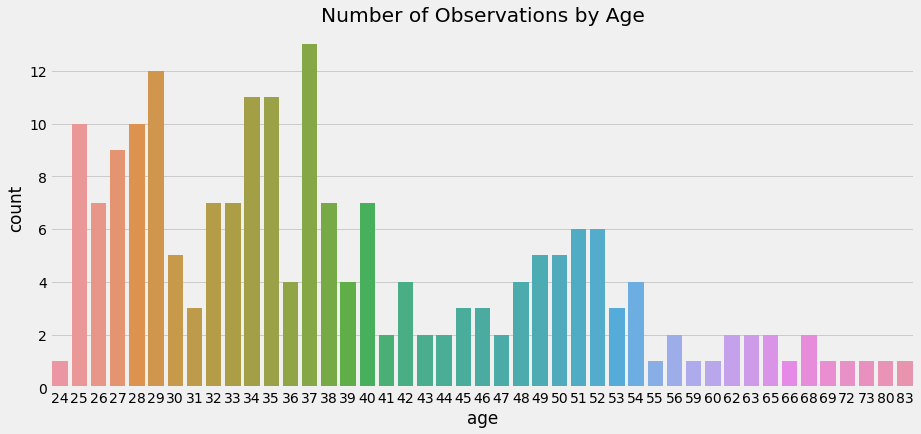
\includegraphics[width=10cm]{figures/age-general-view.png}}
        \caption{\label{fig:age-general-view} Age stats}
    \end{figure}
    \newpage


    %%%%%%%%%%%%%%%%%%%%%%%%%%%%%%%%%%%%%%%%%%%%%%
    % References
    %%%%%%%%%%%%%%%%%%%%%%%%%%%%%%%%%%%%%%%%%%%%%%


    \section{References}
    \subsection{Glossary}
    \paragraph{1}
    https://www.facebook.com/WebMD (2007). Benzodiazepine Abuse. [online] WebMD. Available at: https://www.webmd.com/mental-health/addiction/benzodiazepine-abuse\#1.
    \paragraph{2}
    Wikipedia Contributors (2019). Benzodiazepine. [online] Wikipedia. Available at: https://en.wikipedia.org/wiki/Benzodiazepine.
    \subsection{Data set}
    \paragraph{1}
    Wikipedia. (2020). Column (database). \\
    [online] Available at: https://en.wikipedia.org/wiki/Column\_(database) [Accessed 11 May 2020].
    \subsection{Pre-processing}
    \paragraph{1}
    Yarlagadda, A., Murthy, J.V.R. and Krishna Prasad, M.H.M. (2015). A novel method for human age group classification based on Correlation Fractal Dimension of facial edges. Journal of King Saud University - Computer and Information Sciences, [online] 27(4), pp.468\textendash{}476. Available at: https://www.sciencedirect.com/science/article/pii/S1319157815000671 [Accessed 7 Jul. 2019].

\end{document}
